\documentclass[aspectratio=169]{beamer}

\usetheme{AnnArbor}
\setbeamertemplate{navigation symbols}{}

\usepackage[T1]{fontenc}
\usepackage[utf8]{inputenc}
\usepackage{graphicx}
\usepackage{booktabs}

\title[UM ParkSight]{UM ParkSight: Vision-Based Parking Occupancy Estimation}
\subtitle{Reference-Image Registration for U-M Lots}
\author{Felix Sixiang Tang \and Keheng Zhu \and Kwan Ting Lau}
\institute{EECS 504}
\date{April 2026}

\begin{document}

\begin{frame}
    \titlepage
\end{frame}

\begin{frame}{Problem and Goal}
\begin{itemize}
    \item Parking search increases congestion, delay, and emissions.
    \item Existing solutions either lack per-space detail (gate counters) or require expensive hardware (per-space sensors).
    \item Goal: infer per-spot occupancy from a single oblique lot photo.
    \item Constraint: low-cost setup with one-time calibration per lot.
\end{itemize}
\end{frame}

\begin{frame}{System Overview}
\begin{columns}[T]
    \column{0.54\textwidth}
    \begin{itemize}
        \item One-time reference annotation defines spot polygons.
        \item LoFTR + homography transfers spots to query images.
        \item Per-spot crops are classified as occupied/empty.
        \item Output is a glanceable occupancy map.
    \end{itemize}

    \column{0.46\textwidth}
    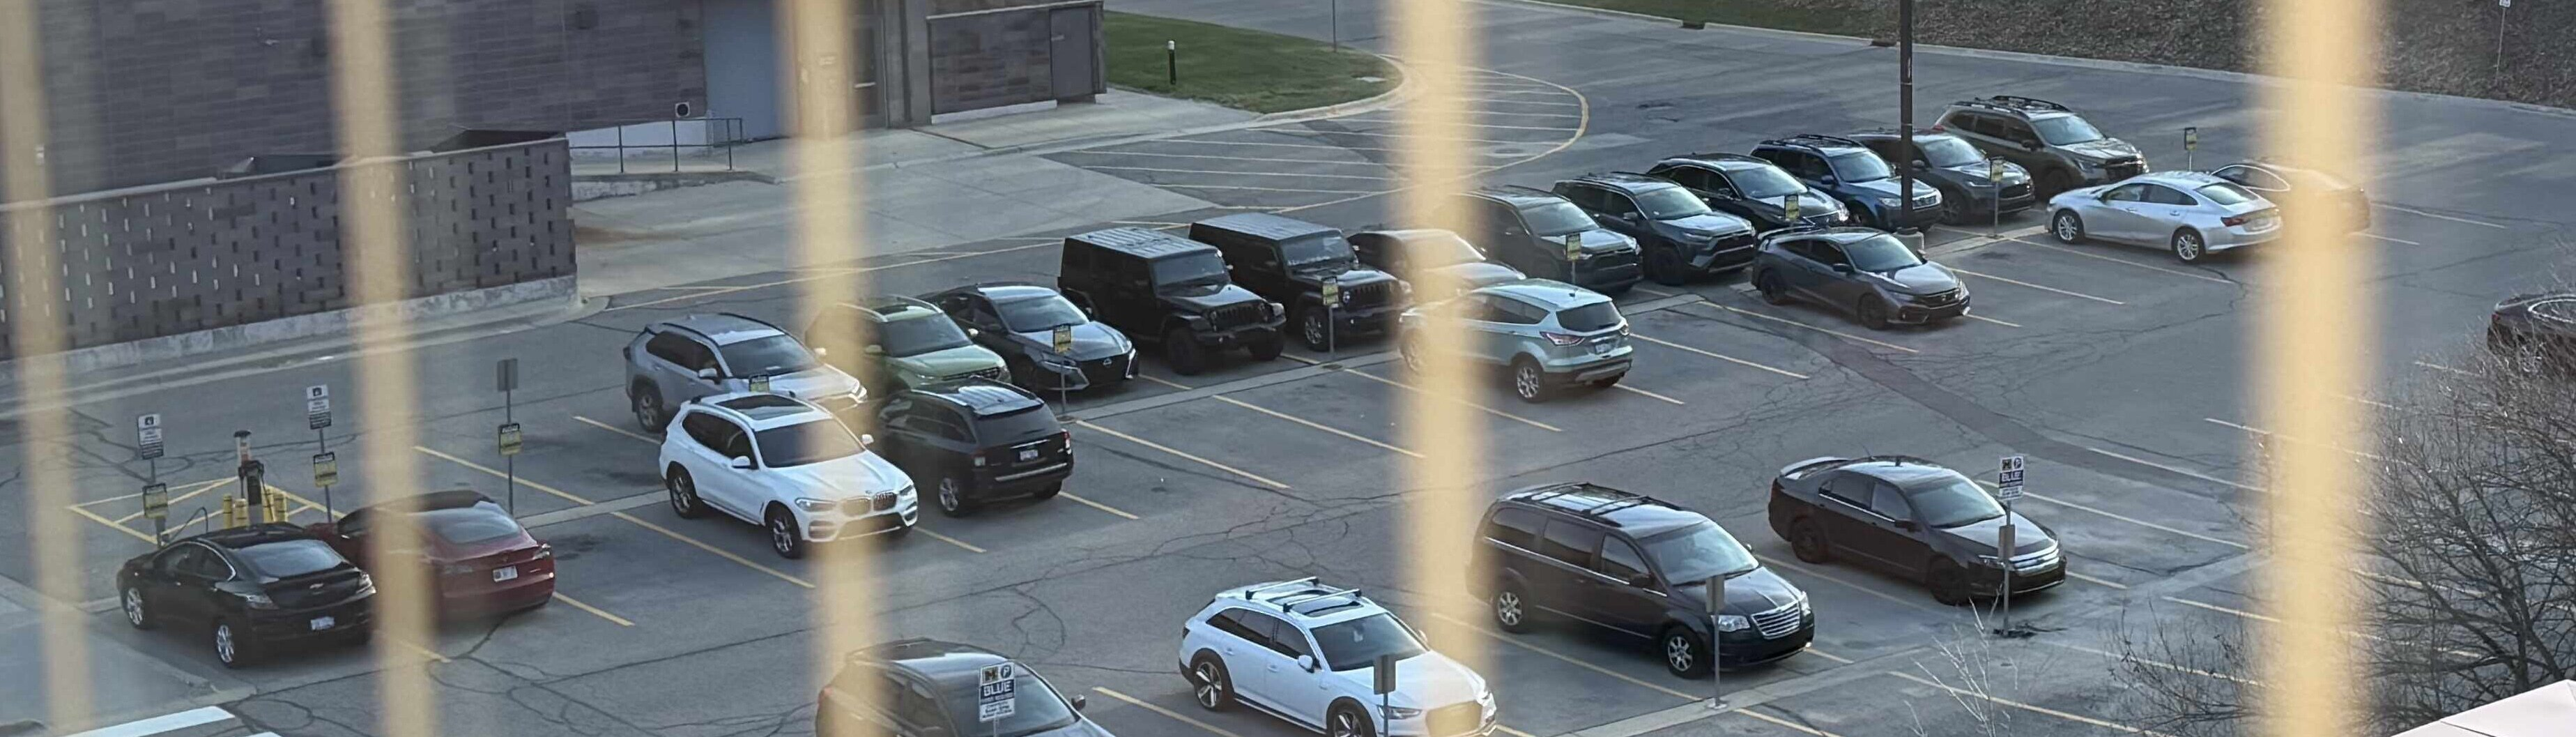
\includegraphics[width=\linewidth]{figures/reference_image.jpg}
    \vspace{0.02\textheight}
    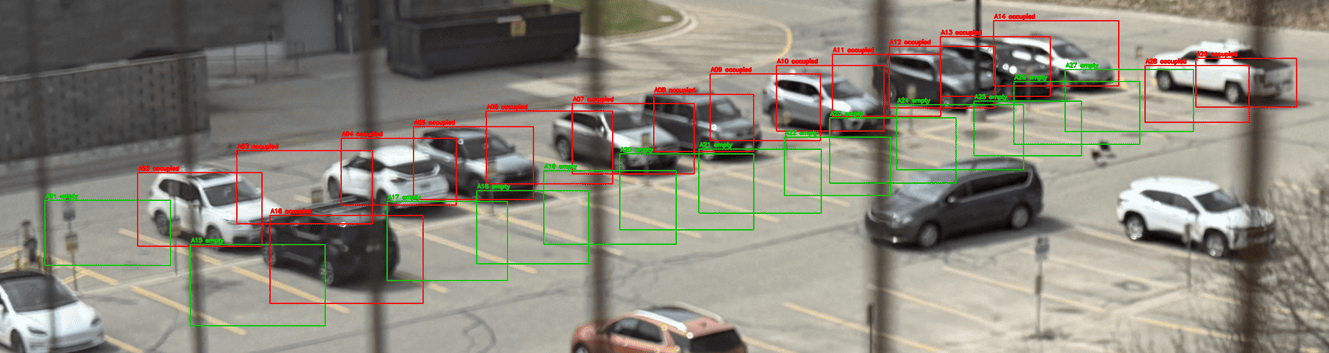
\includegraphics[width=\linewidth]{figures/resolved_occupancy_overlay.png}
\end{columns}
\end{frame}

\begin{frame}{Method: Registration via LoFTR}
\begin{columns}[T]
    \column{0.67\textwidth}
    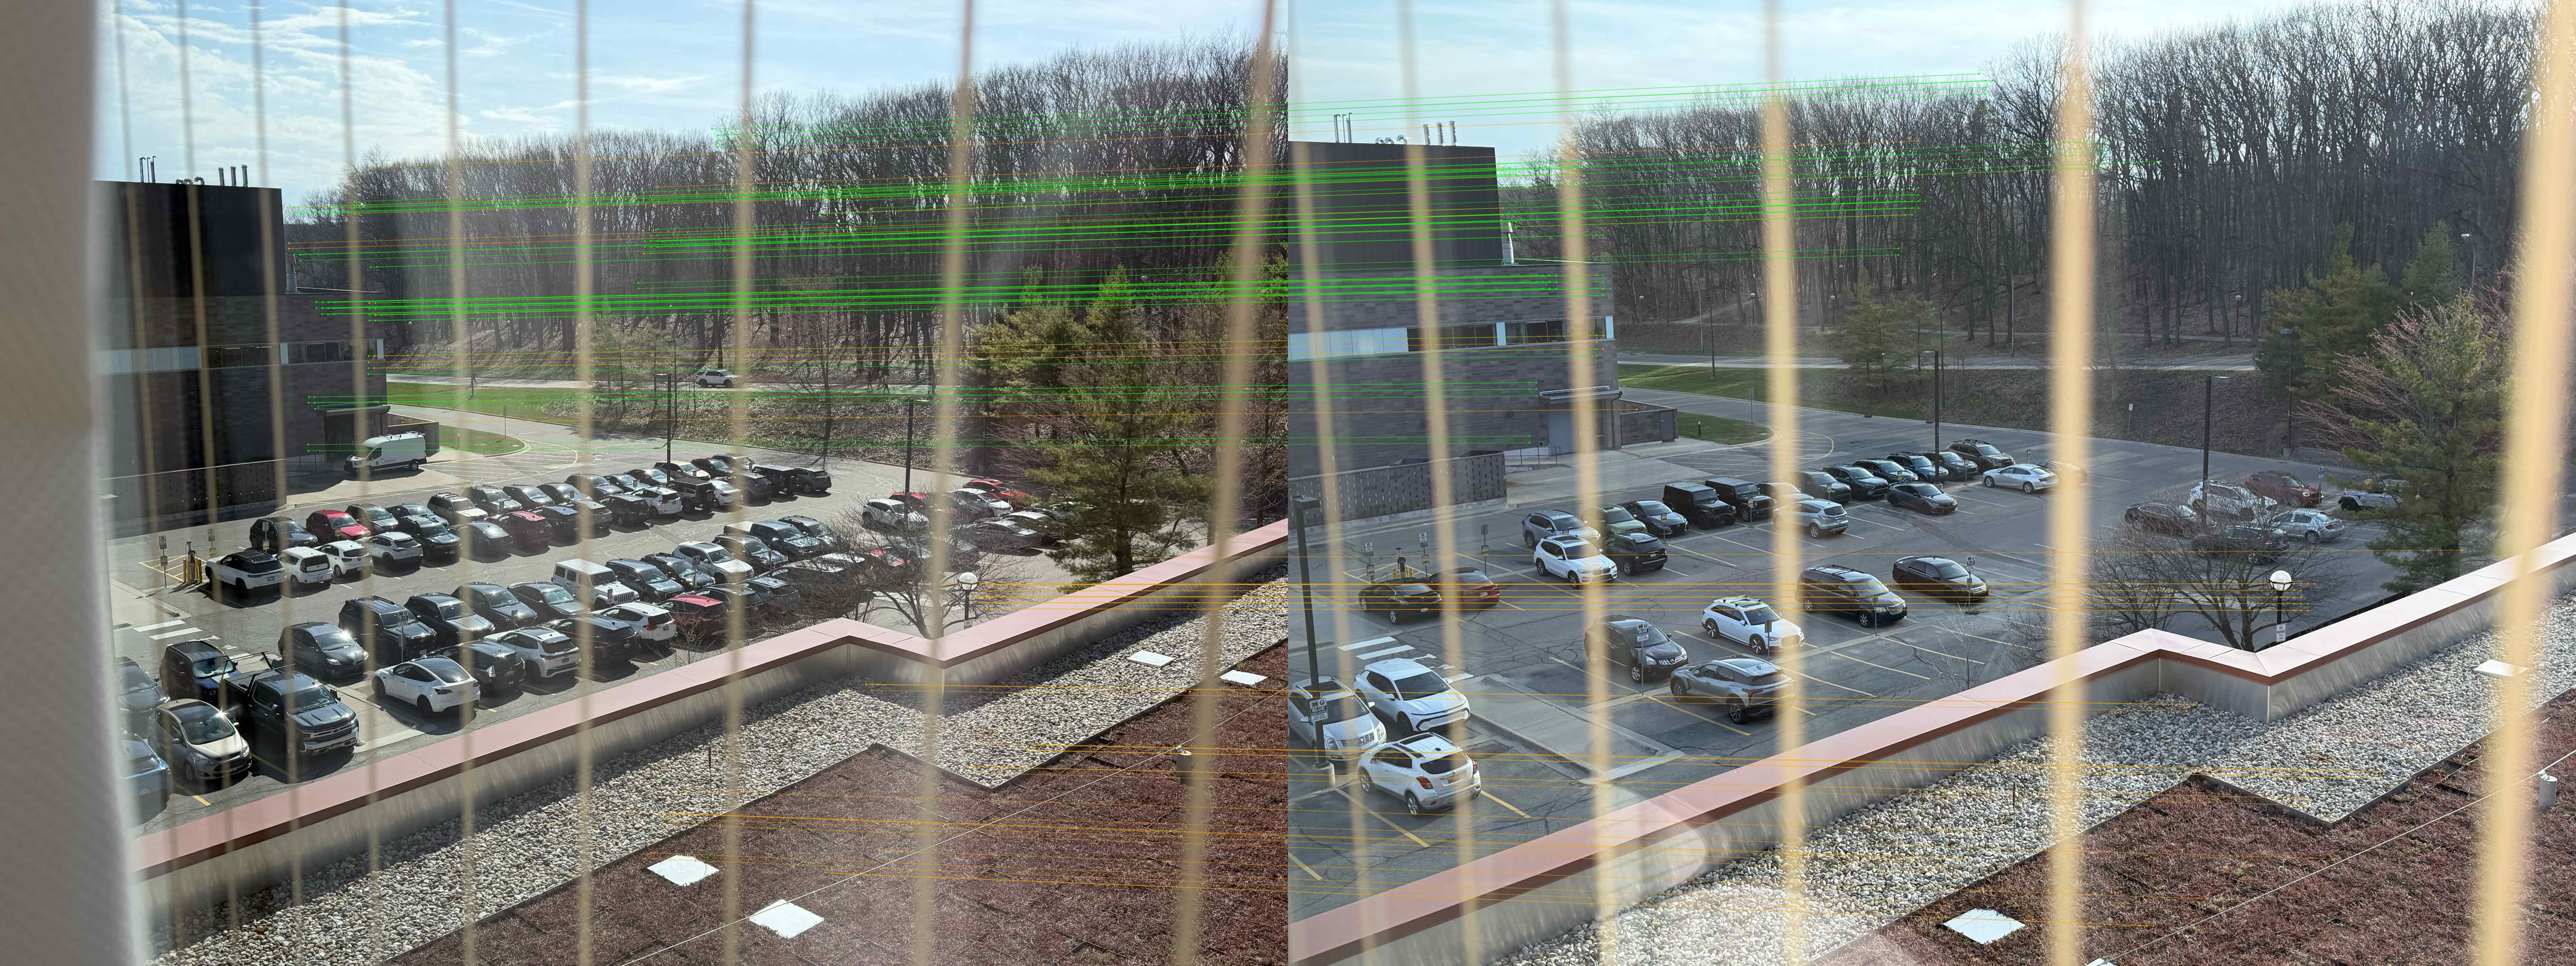
\includegraphics[width=\linewidth]{figures/loftr_matches_query.jpg}

    \column{0.33\textwidth}
    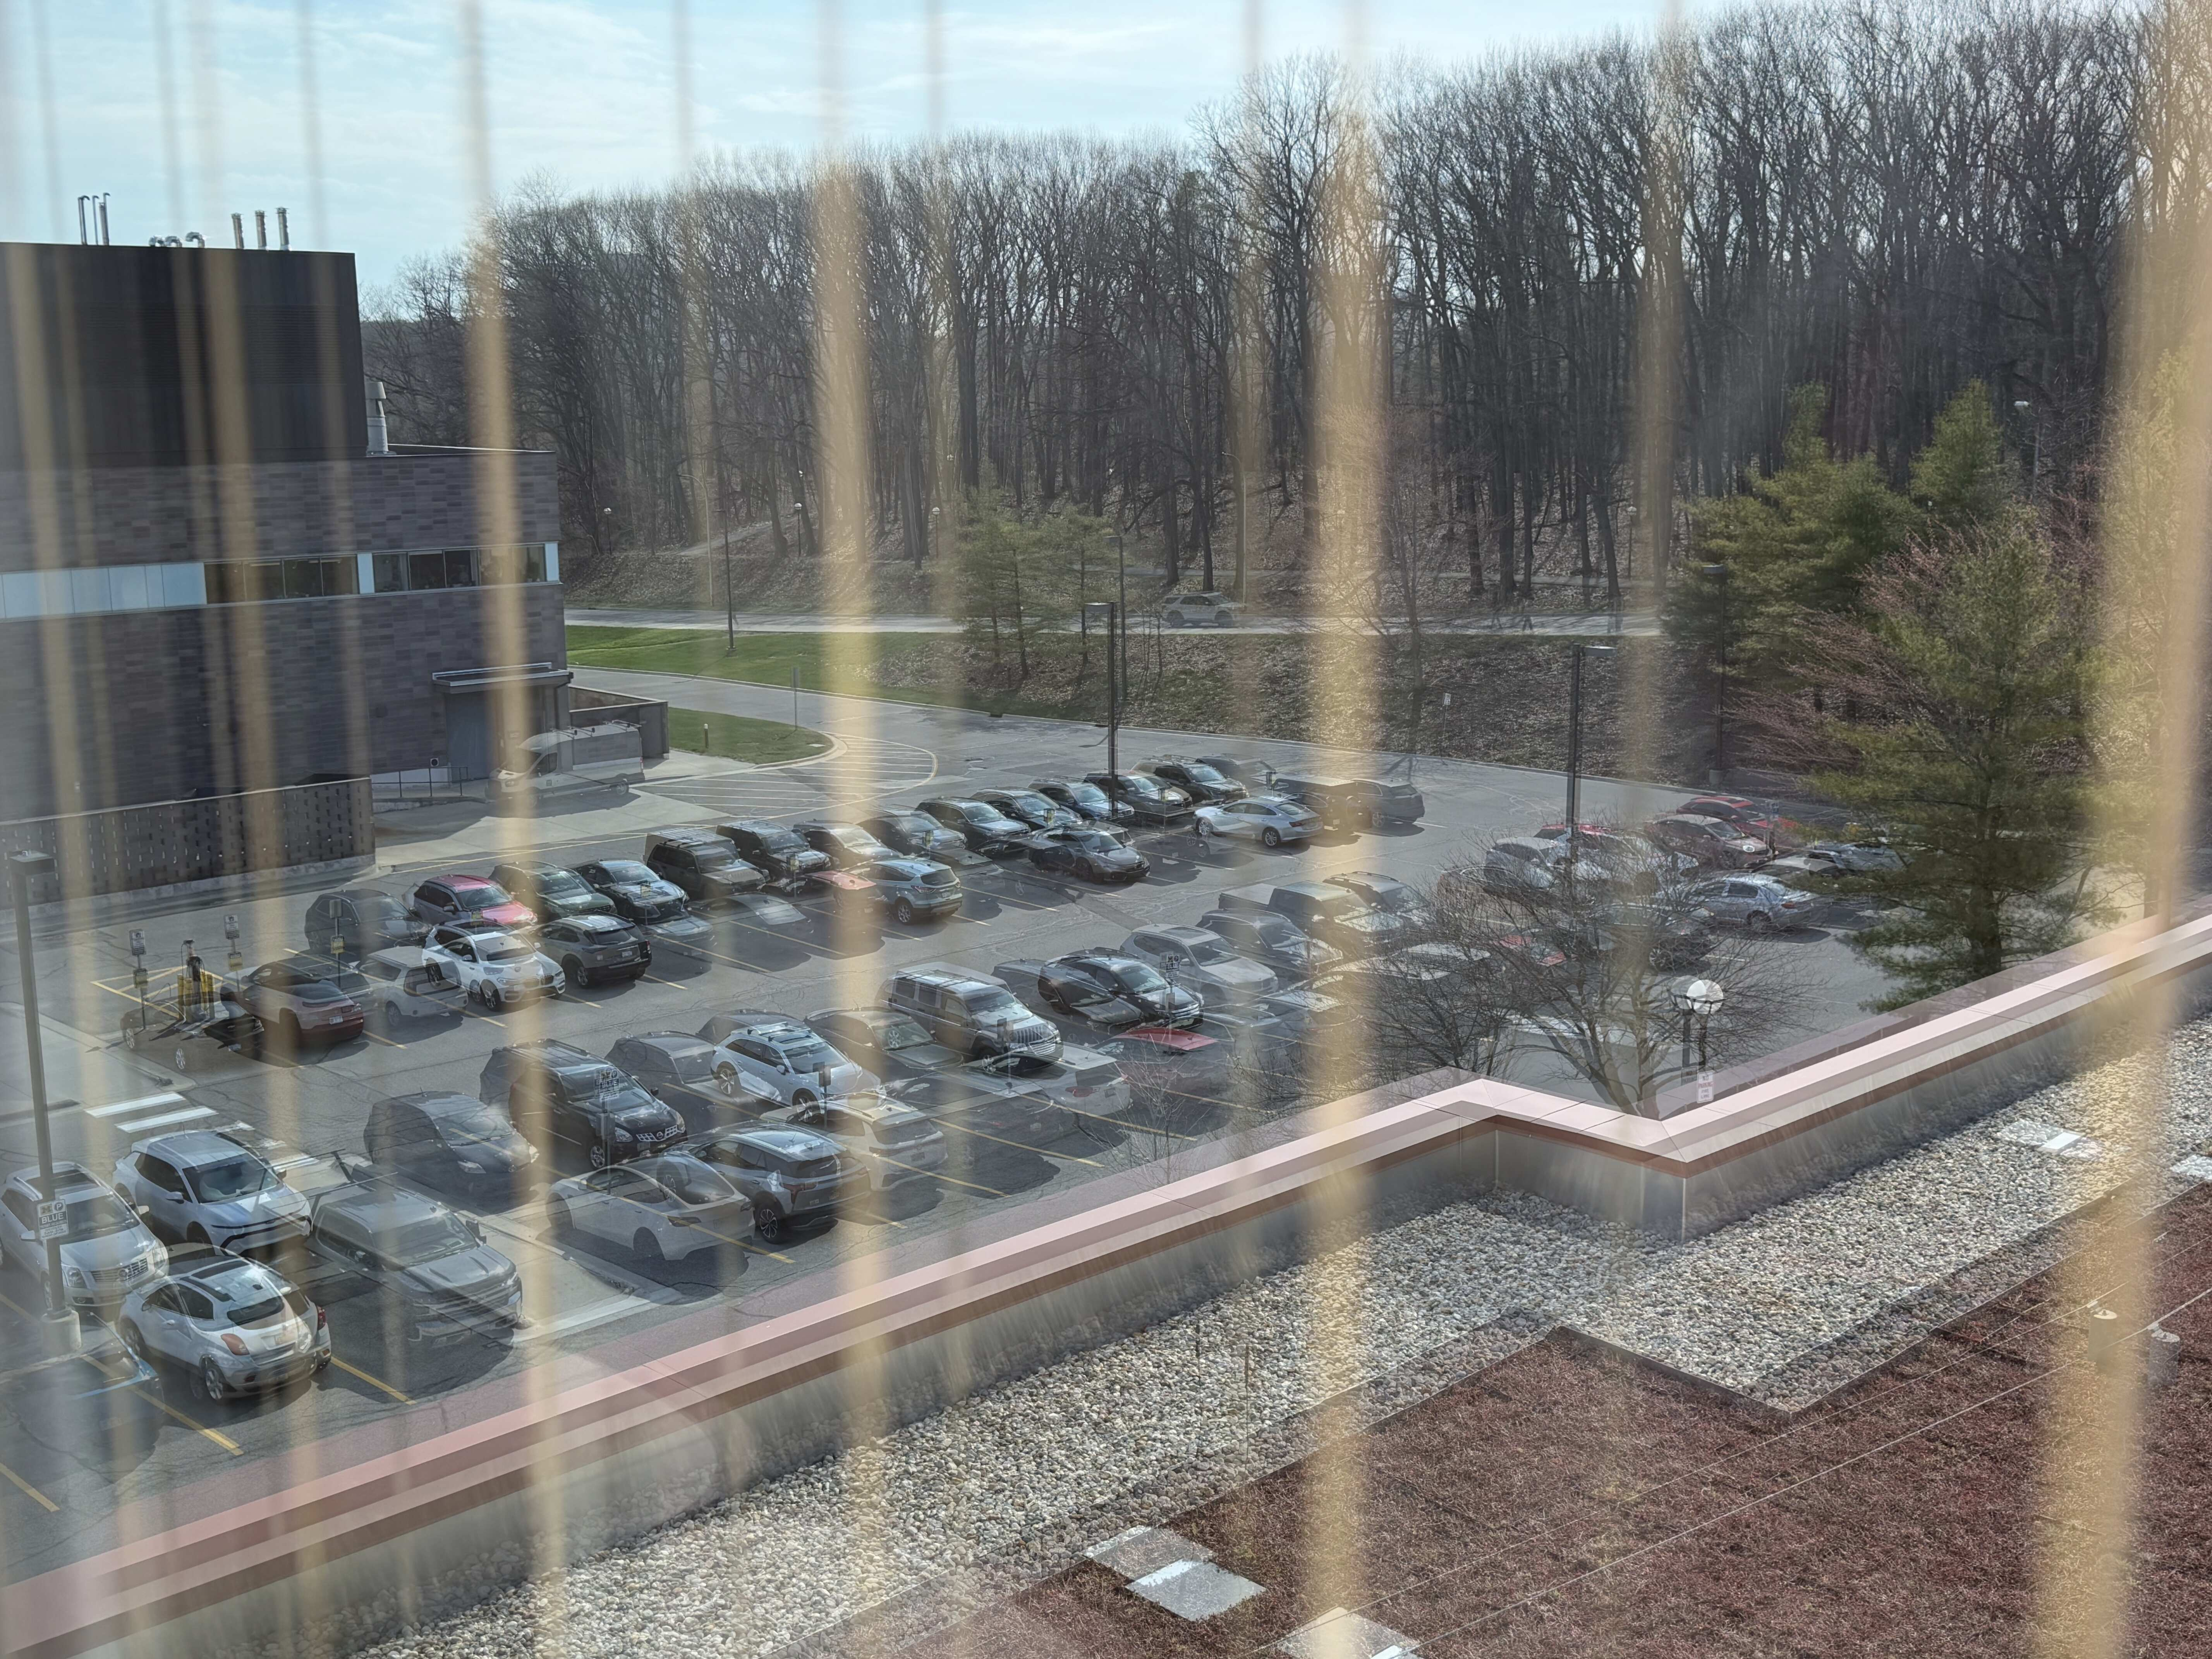
\includegraphics[width=\linewidth]{figures/registration_overlay.jpg}
\end{columns}
\vspace{0.02\textheight}
\begin{itemize}
    \item Dense correspondences in low-texture asphalt regions.
    \item RANSAC homography maps reference coordinates to query frame.
\end{itemize}
\end{frame}

\begin{frame}{Method: Per-Spot Classification}
\centering
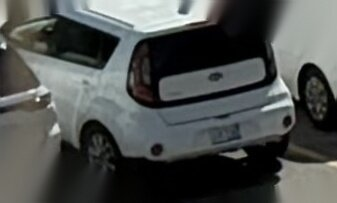
\includegraphics[width=0.31\textwidth]{figures/spot_occupied_example.jpg}\hfill
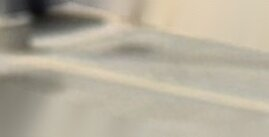
\includegraphics[width=0.31\textwidth]{figures/spot_empty_example.jpg}\hfill
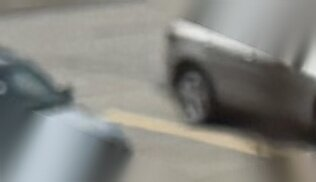
\includegraphics[width=0.31\textwidth]{figures/spot_borderline_example.jpg}
\vspace{0.03\textheight}
\begin{itemize}
    \item Each warped spot polygon is cropped and scored by the detector.
    \item Rule-based gating uses confidence, center alignment, and area ratio.
\end{itemize}
\end{frame}

\begin{frame}{Method: End-User 2D Occupancy Map}
\centering
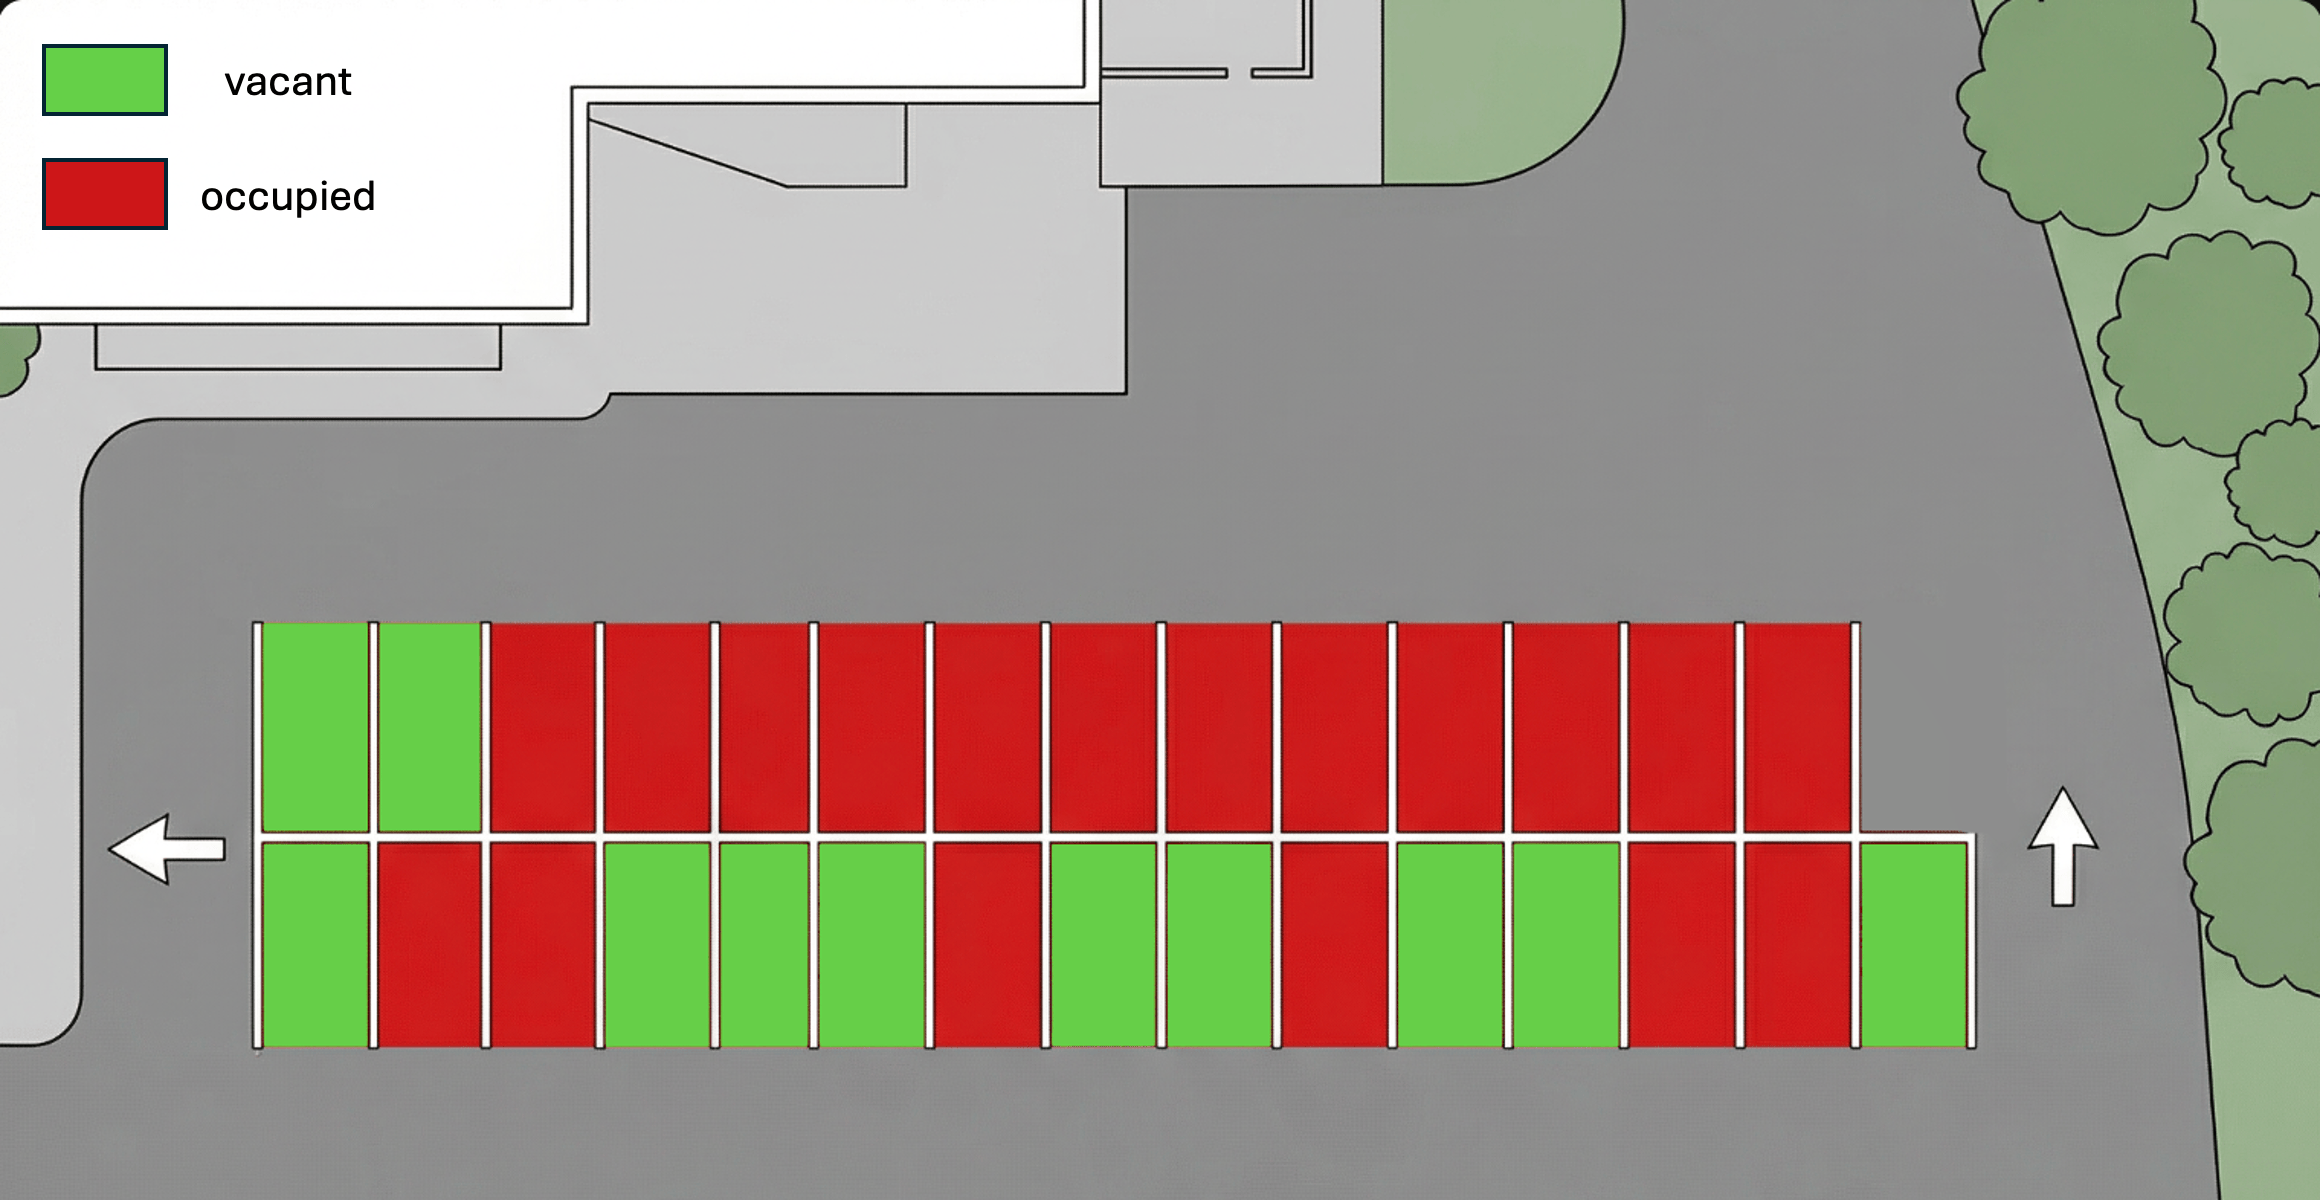
\includegraphics[width=0.72\textwidth]{figures/2D_map.png}
\vspace{0.02\textheight}

Green = available, red = occupied; designed for fast phone-based lookup.
\end{frame}

\begin{frame}{Prototype Iteration: What Failed First}
\centering
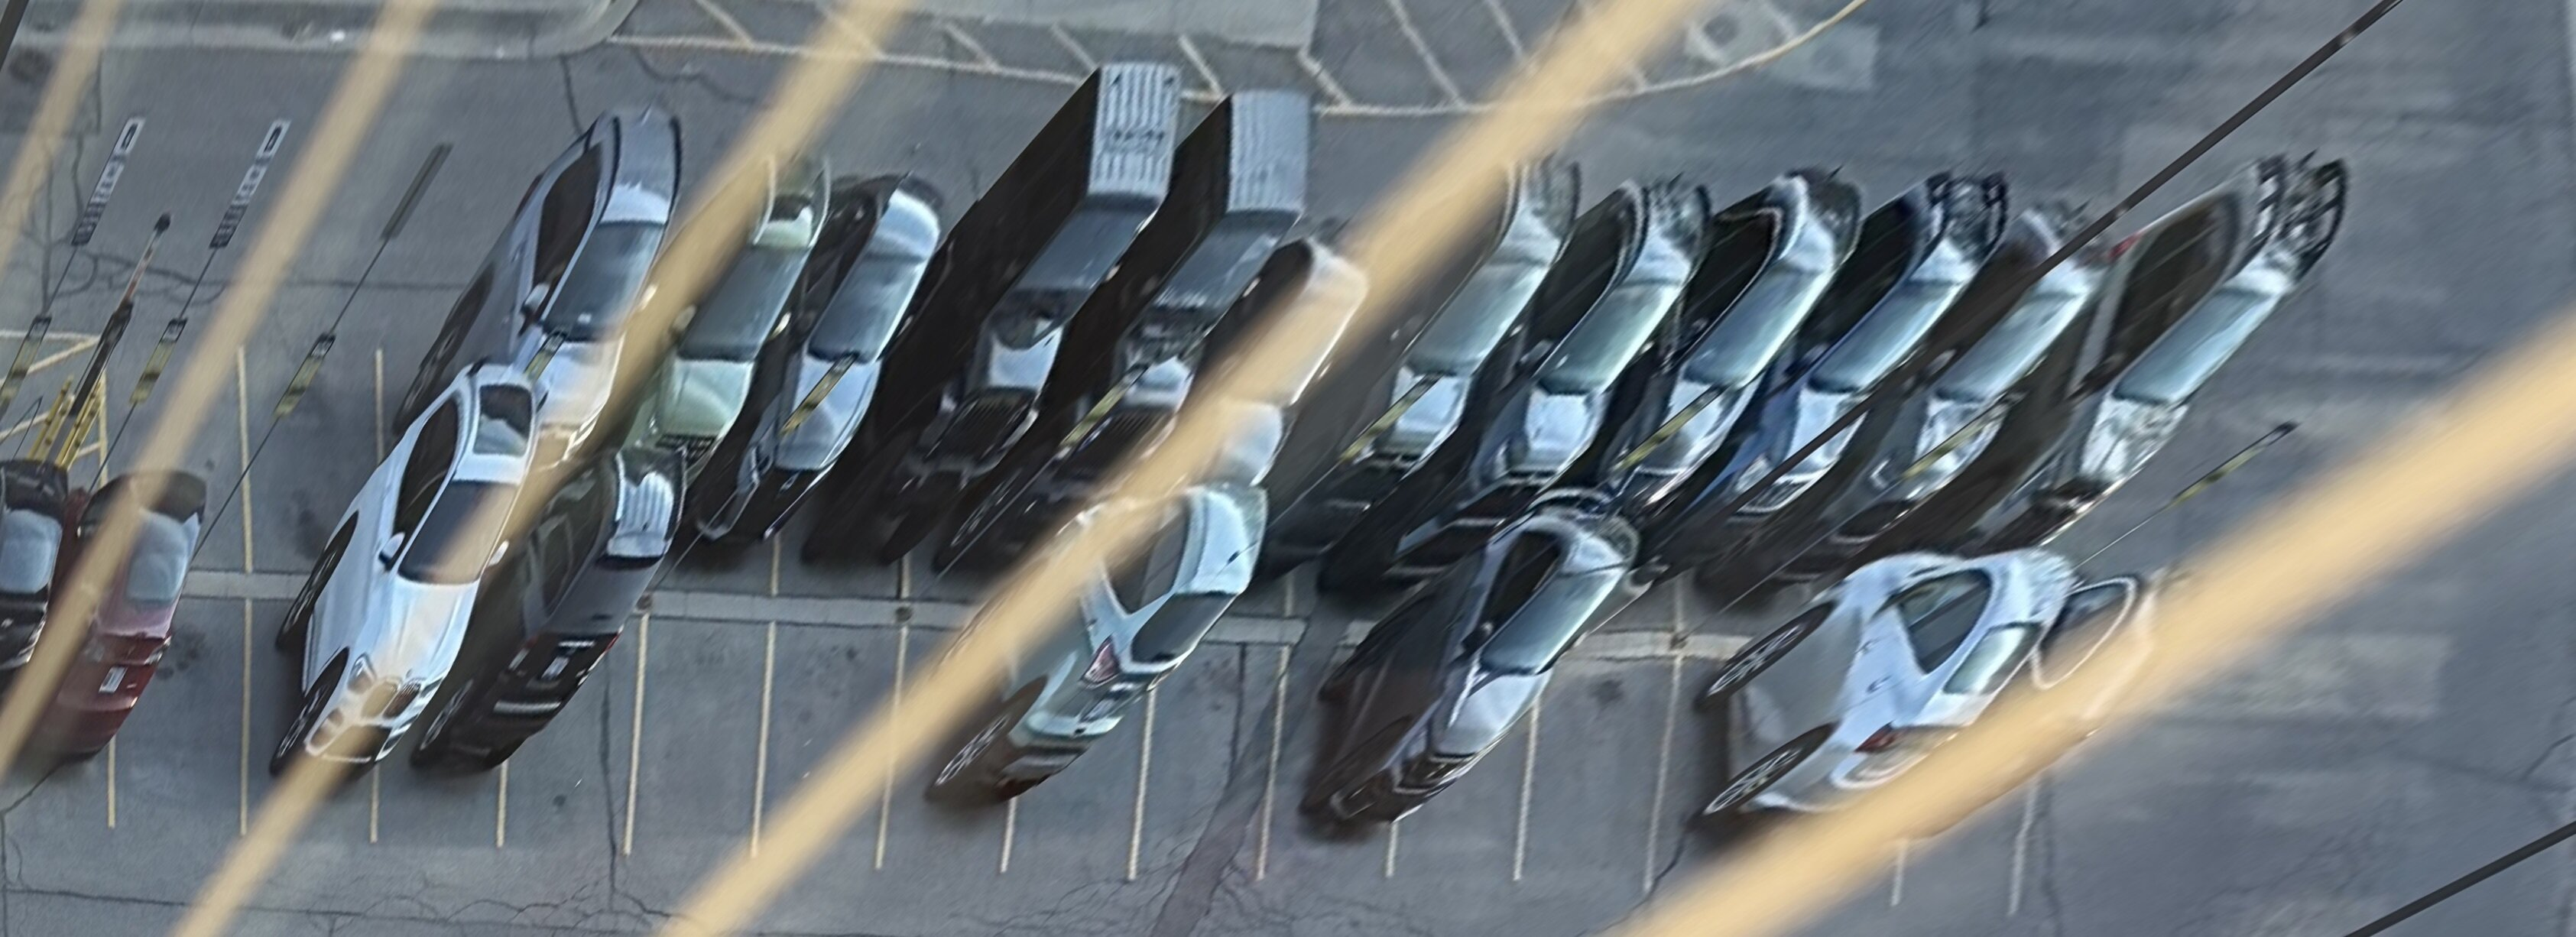
\includegraphics[width=0.48\textwidth]{figures/prototype_direct_detection_failure.jpg}\hfill
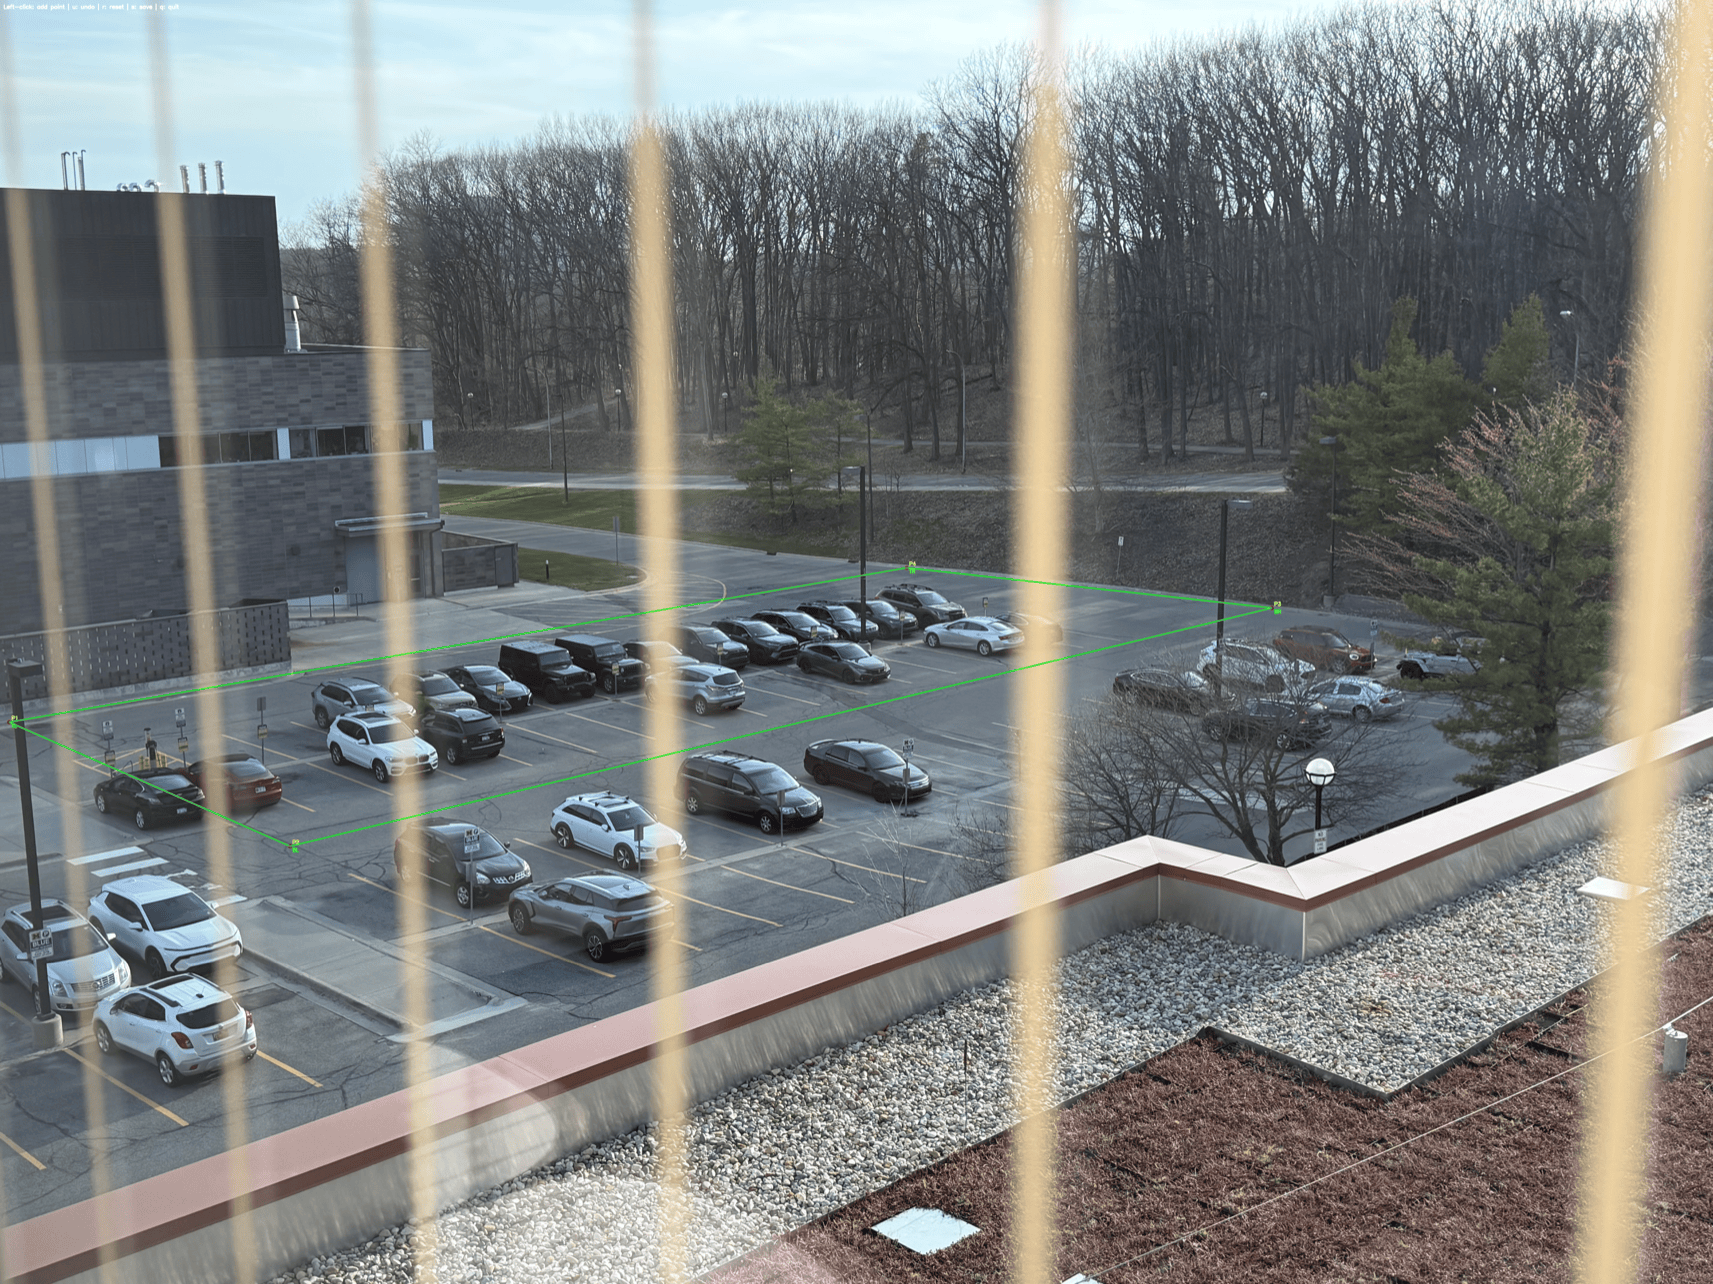
\includegraphics[width=0.48\textwidth]{figures/prototype_line_detection_failure.png}
\vspace{0.03\textheight}
\begin{itemize}
    \item Direct car detection on oblique scenes was unstable.
    \item Automated parking-line extraction failed under occlusion and faded markings.
\end{itemize}
\end{frame}

\begin{frame}{Results: Spot-Level Detection Grid}
\centering
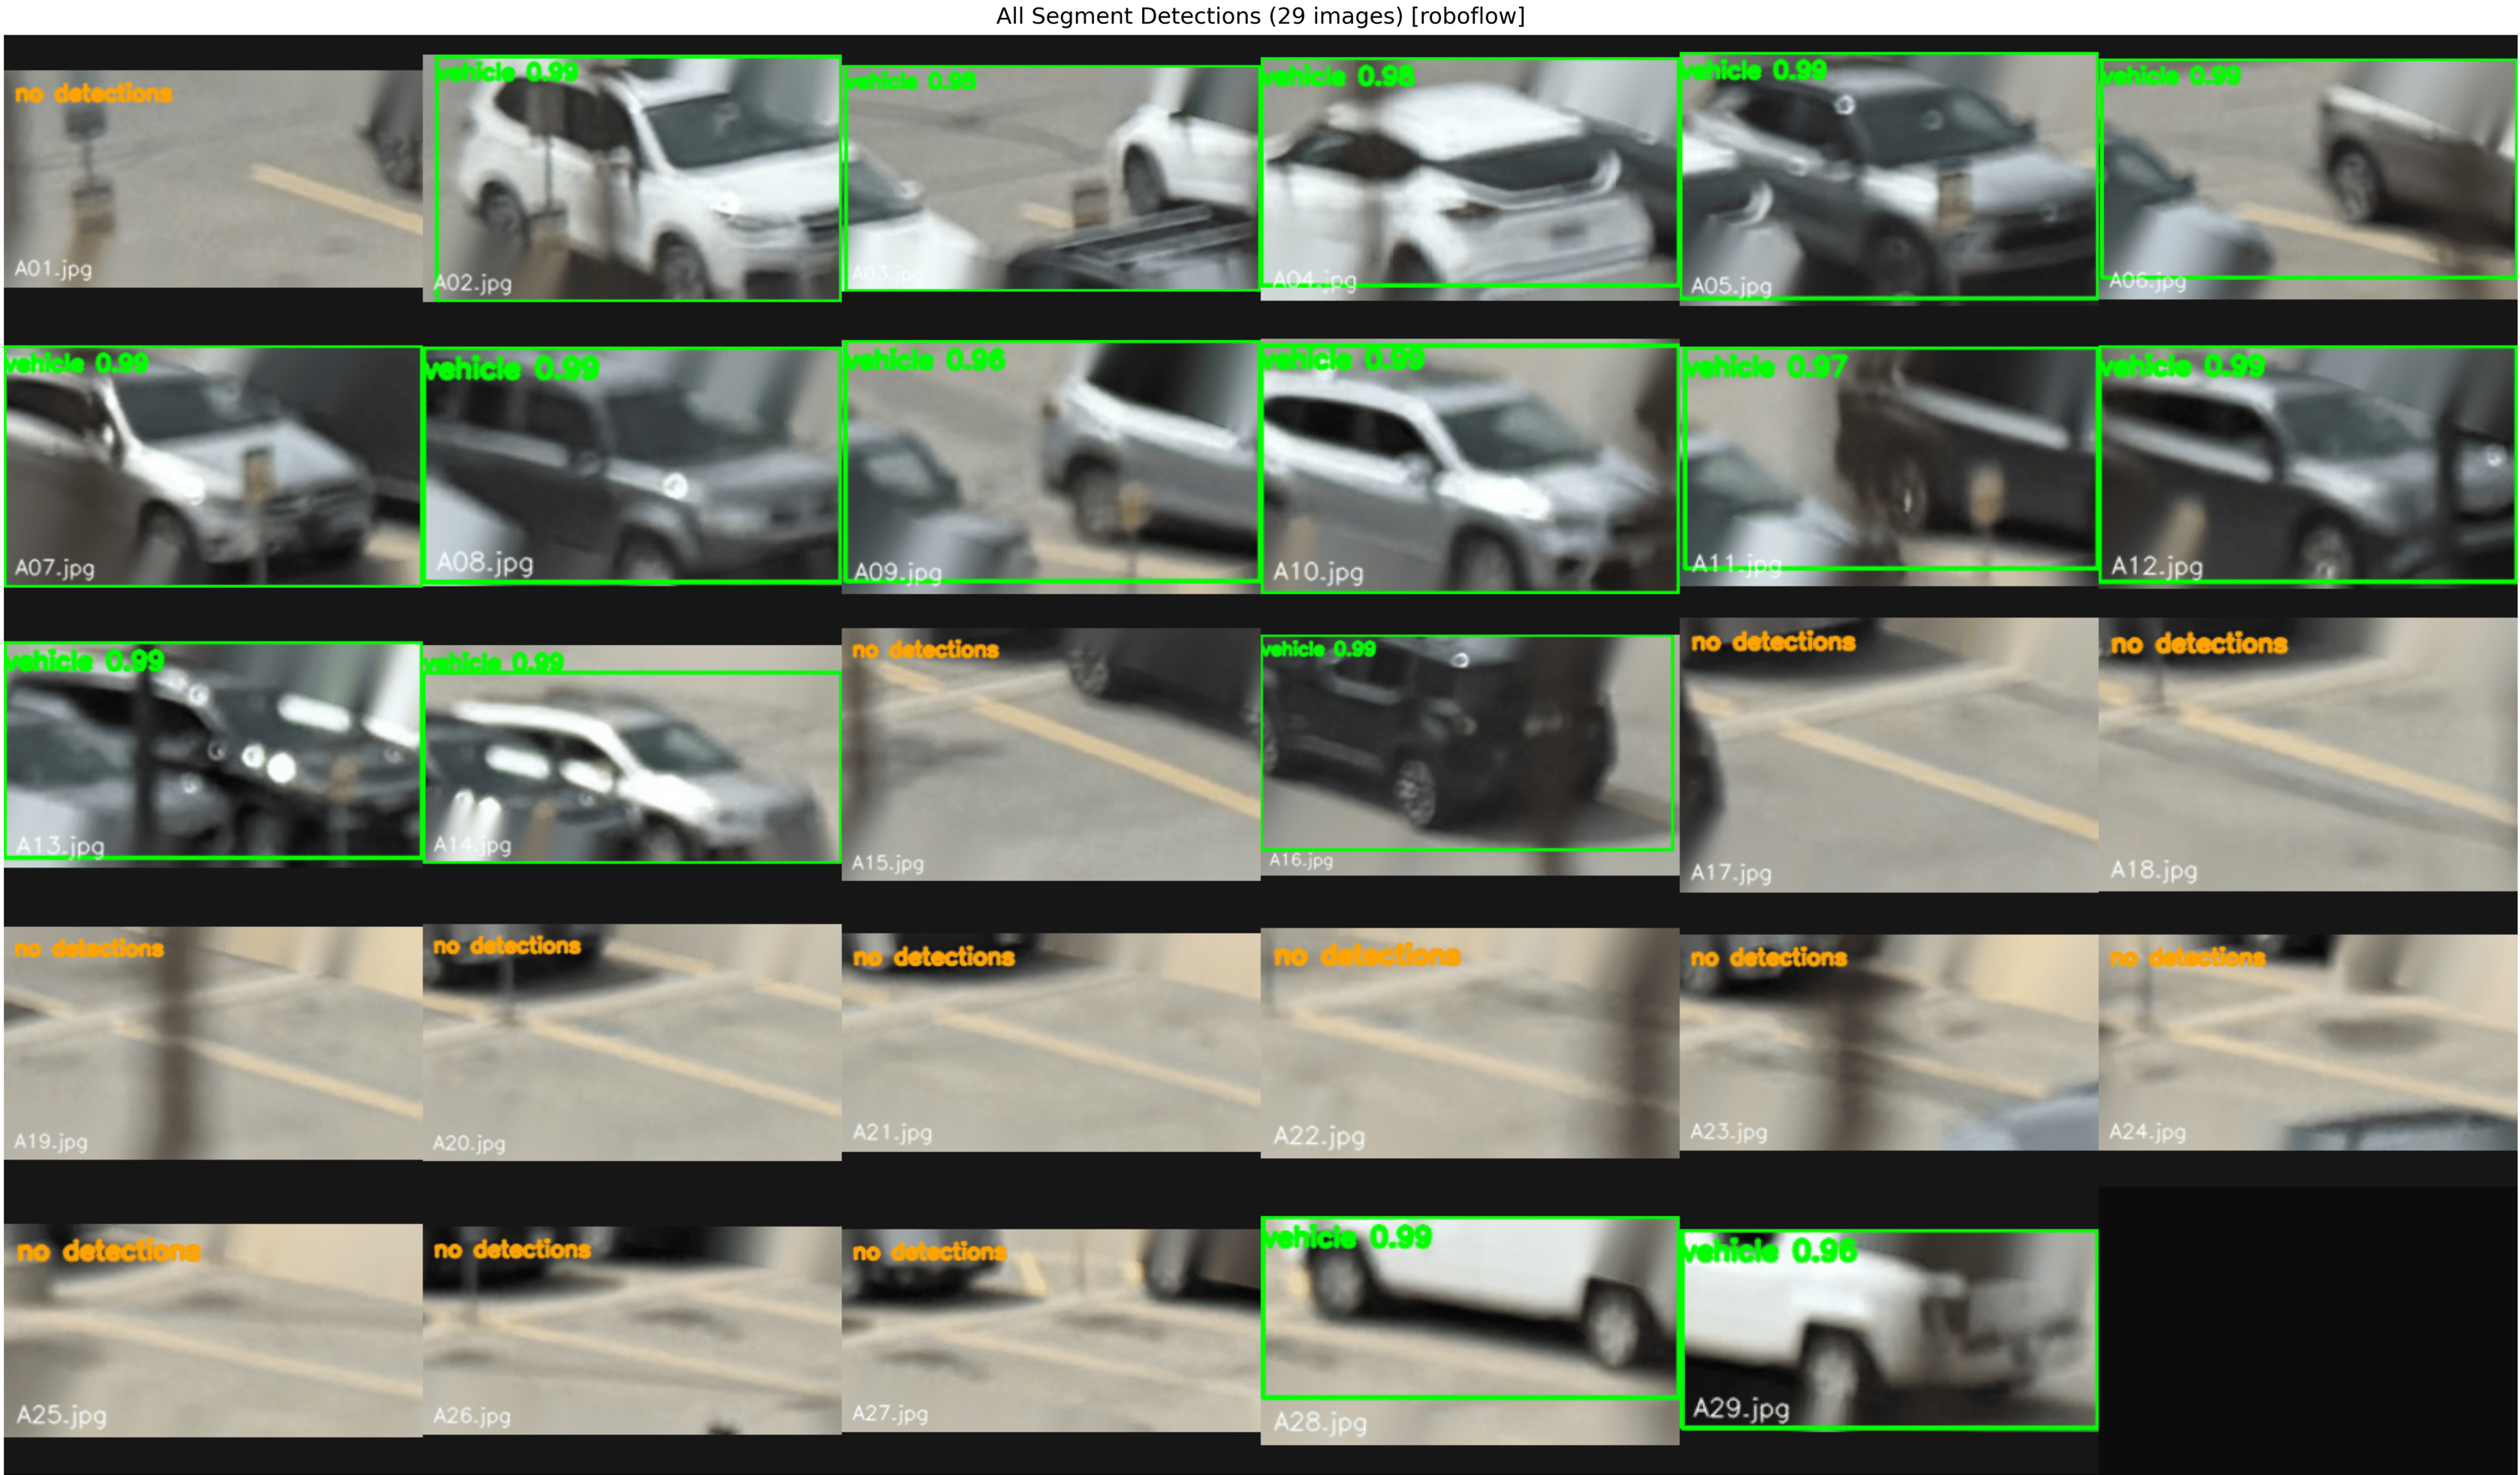
\includegraphics[width=0.95\textwidth]{figures/segment_detection_grid.png}
\vspace{0.02\textheight}

29 spot crops are evaluated in a single batch for occupancy evidence.
\end{frame}

\begin{frame}{Results: Registration Consistency Across Queries}
\centering
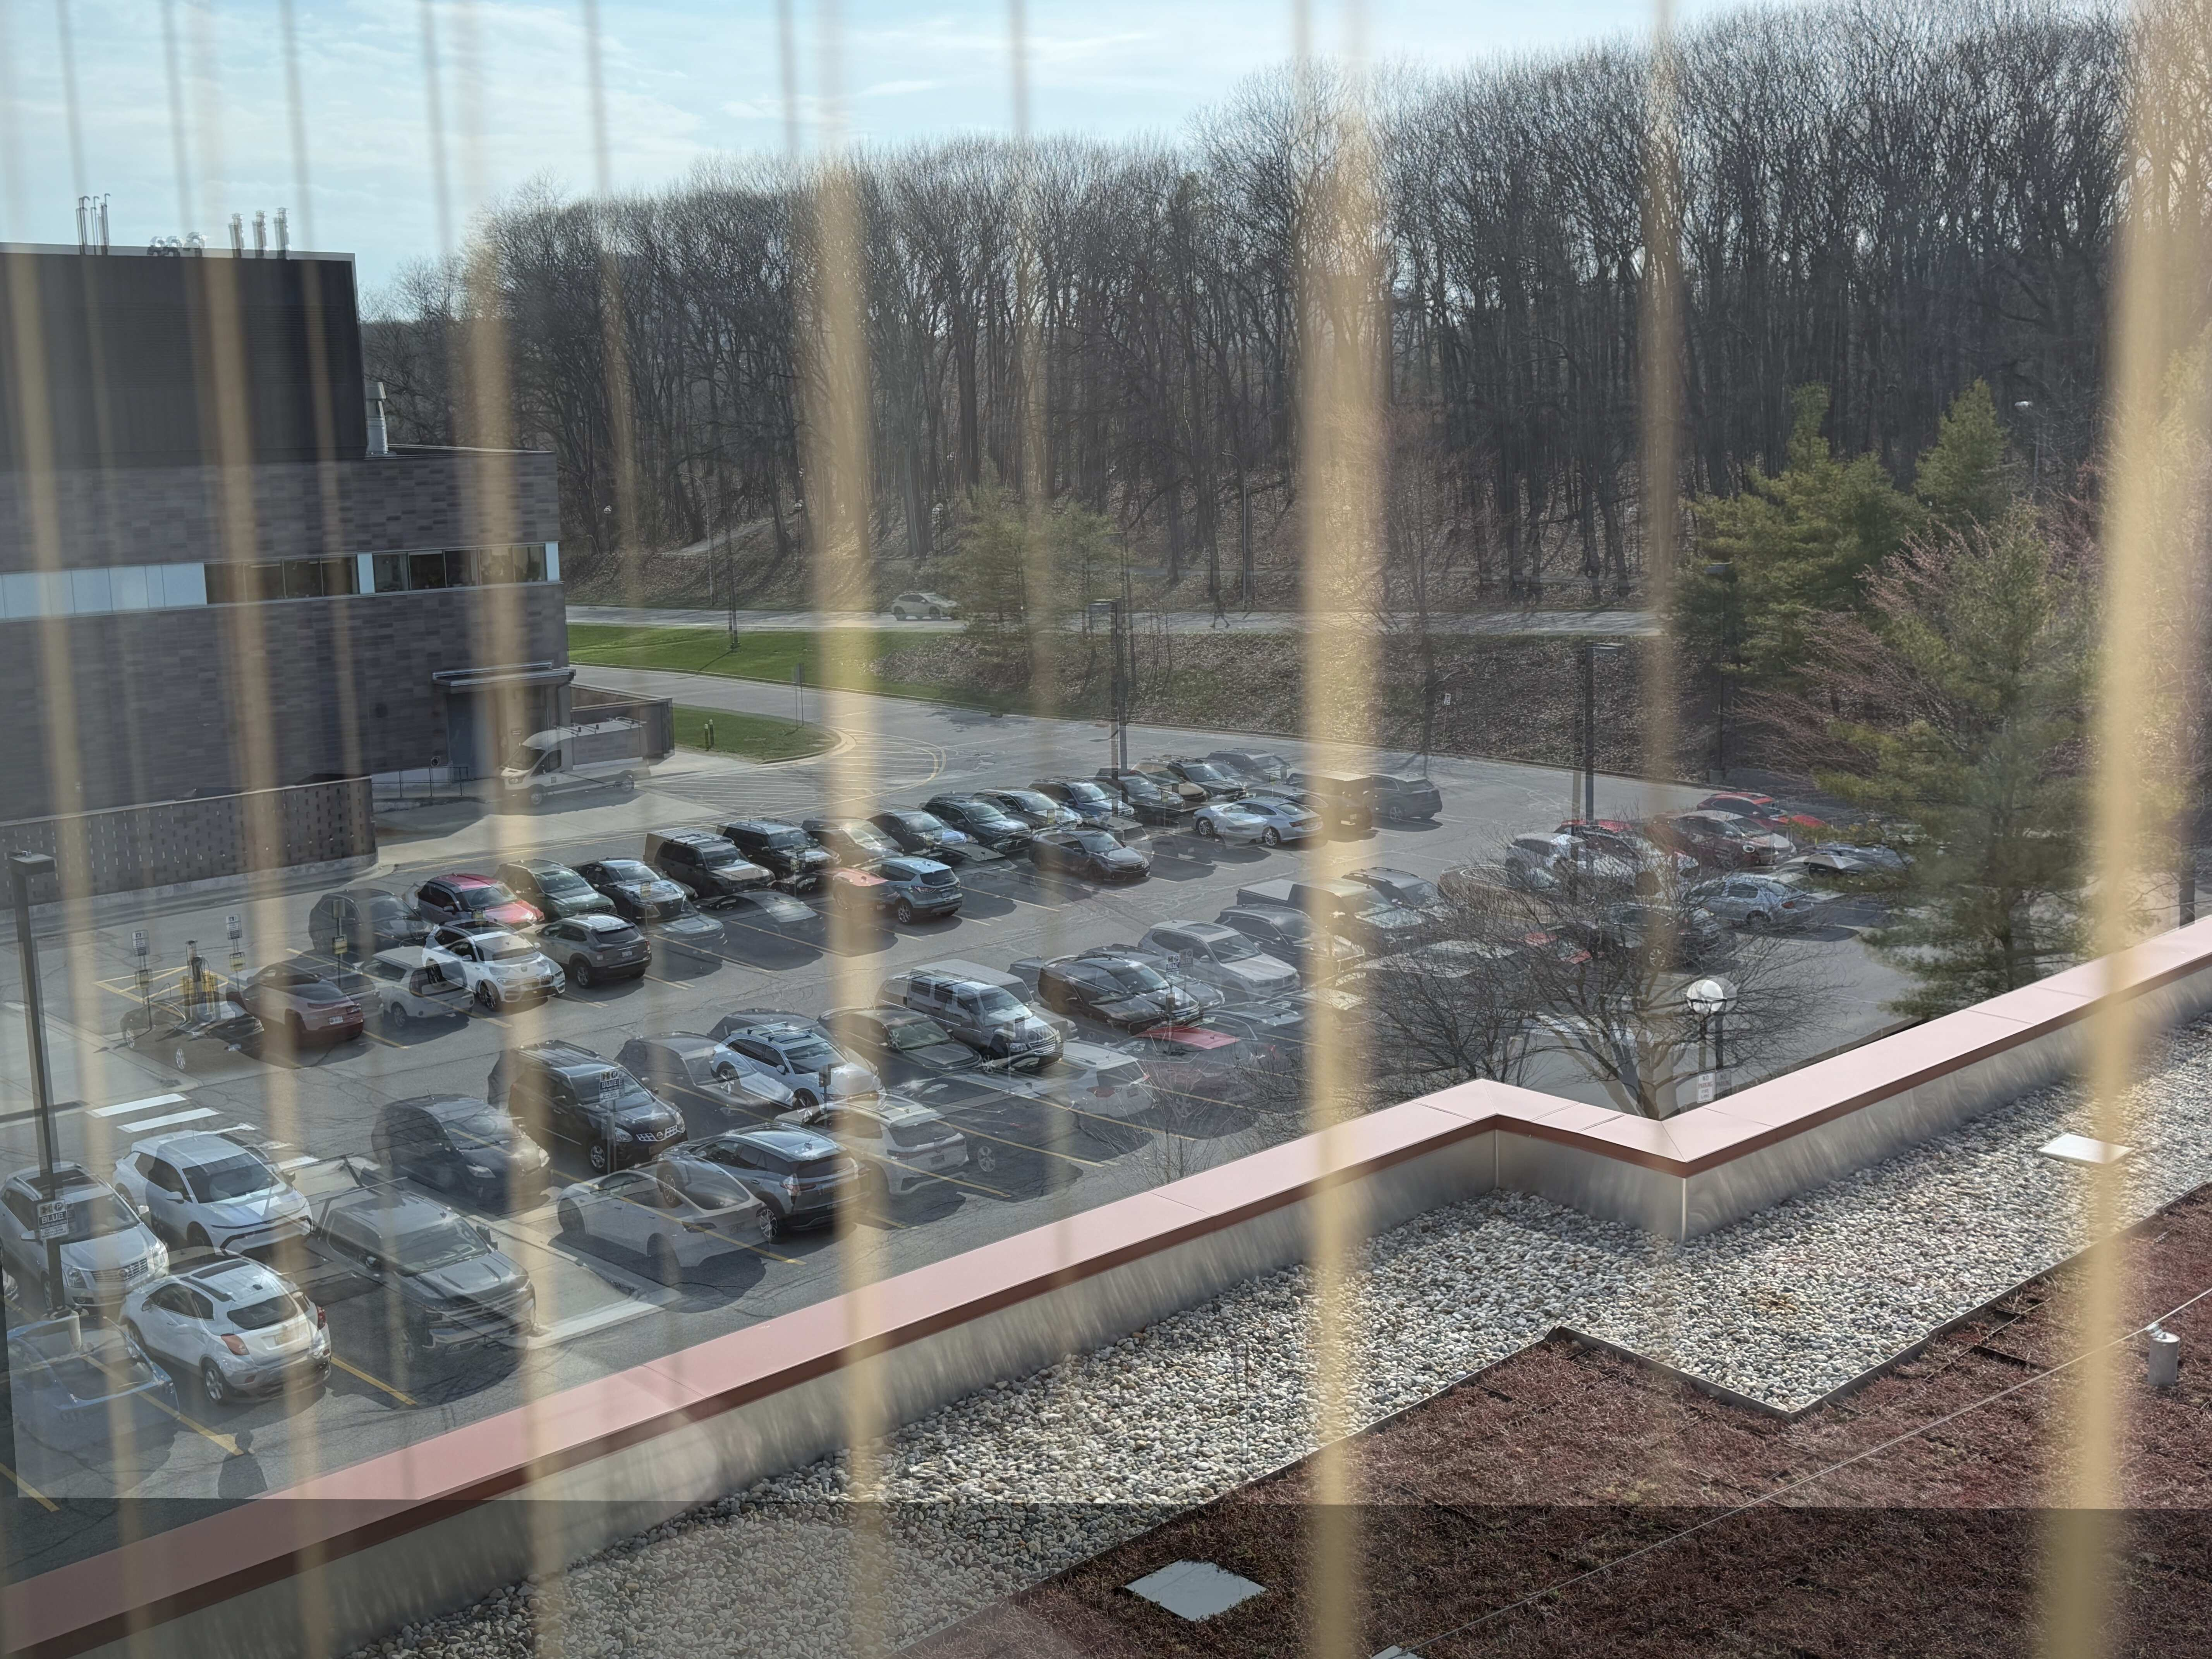
\includegraphics[width=0.48\textwidth]{figures/result_overlay_img3287.jpg}\hfill
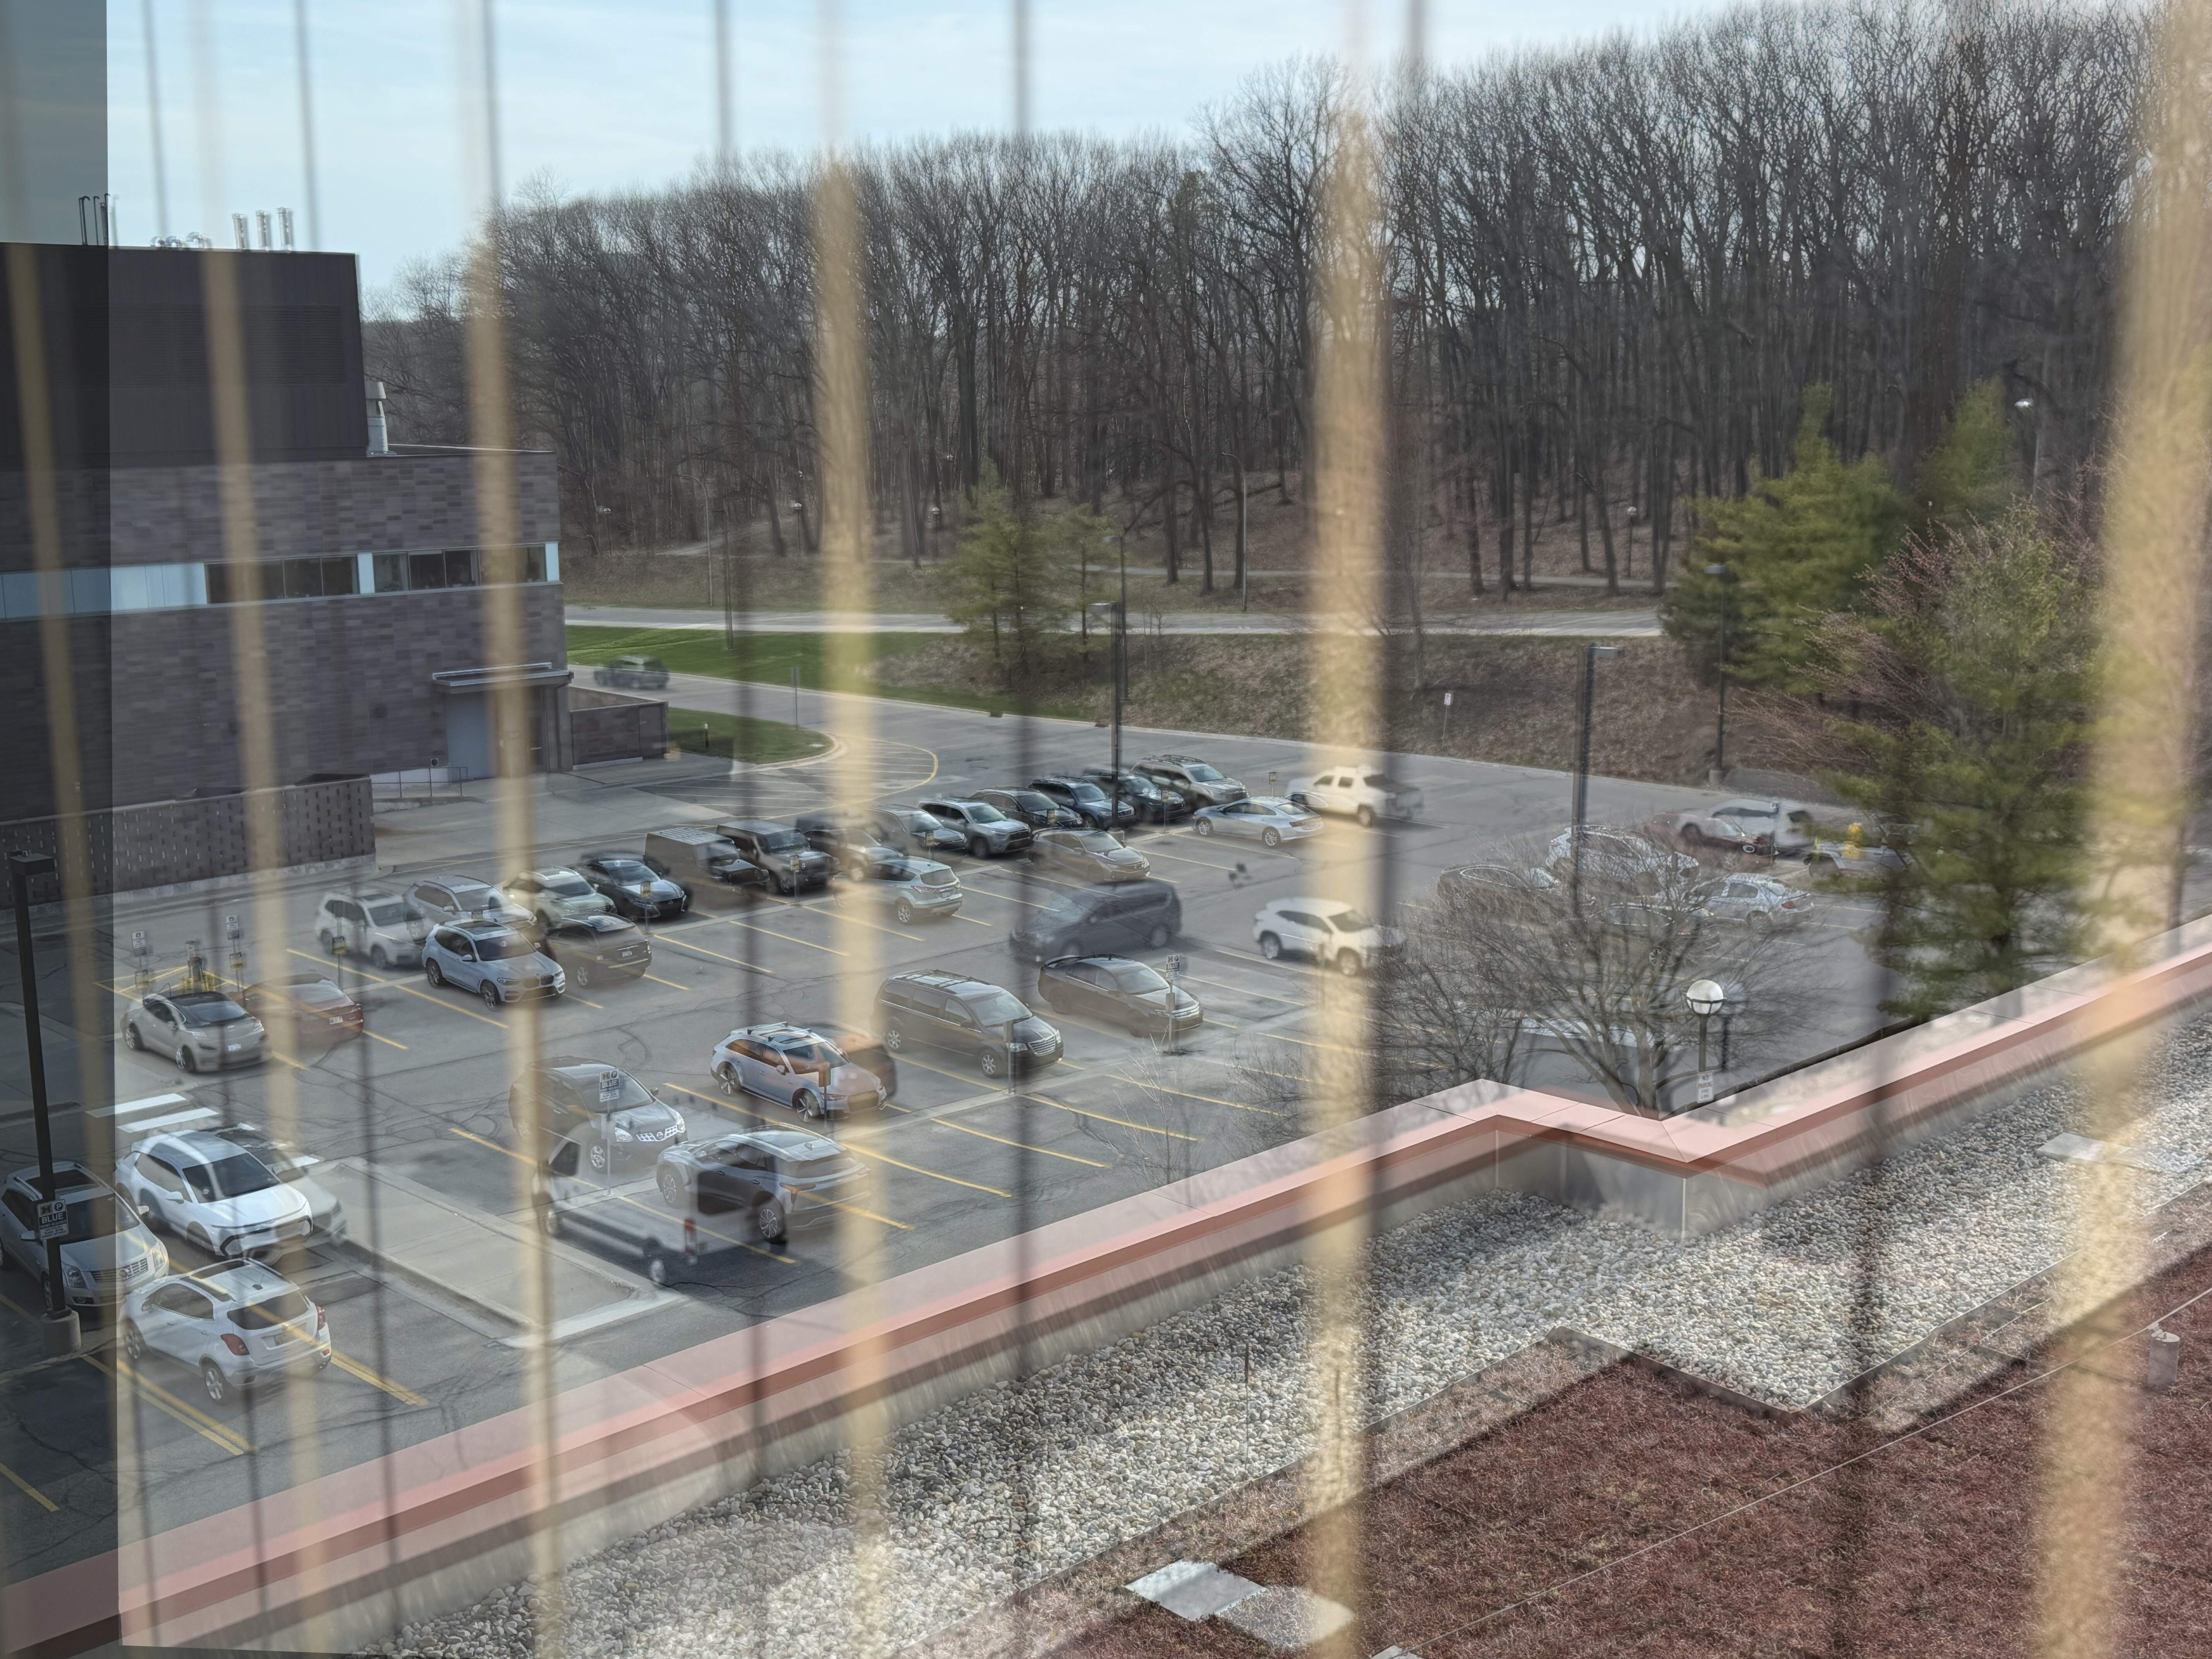
\includegraphics[width=0.48\textwidth]{figures/result_overlay_img3375.jpg}
\end{frame}

\begin{frame}{Results: Quantitative Summary}
\centering
\begin{tabular}{lr}
\toprule
Metric & Value \\
\midrule
Total evaluated spots & 29 \\
Occupied spots & 16 \\
Empty spots & 13 \\
Occupancy rate & 55.17\% \\
Mean occupied confidence & 0.985 \\
Strict-pass occupied spots & 16 / 16 \\
Mean area ratio (strict-pass occupied) & 0.937 \\
\bottomrule
\end{tabular}
\vspace{0.04\textheight}

Descriptive metrics only; no ground-truth labels yet for precision/recall/F1.
\end{frame}

\begin{frame}{Limitations and Next Steps}
\begin{itemize}
    \item Current evaluation is limited to one lot and a small query set.
    \item No manually labeled occupancy ground truth for supervised metrics.
    \item Strong assumption of near-planar geometry for homography transfer.
    \item Next: larger benchmark, threshold calibration, and robustness under lighting/weather changes.
\end{itemize}
\end{frame}

\begin{frame}{Conclusion}
\begin{itemize}
    \item UM ParkSight provides per-space occupancy with minimal infrastructure.
    \item Reference annotation + registration + per-spot inference is practical and scalable.
    \item The prototype demonstrates stable occupancy decisions in representative scenes.
\end{itemize}

\vfill
\centering
\Large Questions?
\end{frame}

\end{document}
